%
%  version 1, 2016-12-05
%
\documentclass[twocolumn,twoside]{svmultivs_br} %please do not change this line
\usepackage{graphicx}
\usepackage{tabularx}

\title*{Norwegian Mapping Authority Analysis Center Biennial Report}
\subtitle{2021--2022}
\titlerunning{NMA AC 2021--2022}

\author{Ann-Silje Kirkvik}
\authorrunning{Kirkvik} % see comments below
\authoremails{ann-silje.kirkvik@kartverket.no}
\institute{Norwegian Mapping Authority (NMA)}

\component{NMA Analysis Center} 

\ContactAuthorName{Ann-Silje Kirkvik}
\ContactAuthorTelephone{+47 32118421}
\ContactAuthorEmail{ann-silje.kirkvik@kartverket.no}
%
\NumberofInstitutions{1}
\InstitutionPostAddress{1}{Postboks 600 Sentrum, 3507 H\onefoss}
\InstitutionCountry{1}{Norway}
\InstitutionWebPage{1}{https://www.kartverket.no}
%
% Example:
%
% \InstitutionPostAddress{1}{61 avenue de l'Observatoire, 75014 Paris}
% \InstitutionCountry{1}{France}
% \InstitutionWebPage{1}{http://www.obspm.fr}
%
\begin{document}  %please do not change this line
%
\maketitle       %please do not change this line
%
\abstract{During 2021 and 2022, the Norwegian Mapping Authority analysis center has contributed to the ITRF2020 
and the operational daily SINEX product. The analysis center has participated in several working groups and 
projects and continued the development of the analysis software \textbf{Where}. The analysis center has also 
investigated the performance of the NYALES20-NYALE13S baseline. The analysis center has successfully transitioned
to the new VLBI naming convention and will continue with its current activities.}
%
\section{General Information}
%
The Norwegian Mapping Authority (NMA) has been an Associate Analysis Center
within the IVS since 2010. The analysis center is operated by the Geodetic
Institute at NMA with the headquarter in H\o nefoss, Norway. NMA is a governmental
agency with approximately 800 employees and the IVS activities at NMA are
completely funded by the Norwegian government.

NMA is using the analysis software \textbf{Where}, which is developed at NMA.
\textbf{Where}\footnote{https://kartverket.github.io/where} and its companion 
library \textbf{Midgard} \footnote{https://kartverket.github.io/midgard} is
freely available as open source at GitHub.
\textbf{Where} is at the moment capable of analyzing single sessions of VLBI data.
Efforts has been made to be able analyze weekly SLR data with \textbf{Where}, but 
this work is currently halted. \textbf{Where} has also been developed to do some 
special analysis within the GNSS domain, but this is not a part of the open source
code.
 
\subsection{Staff}
The Geodetic Institute at NMA is lead by Per Erik Opseth and has approximately 50 employees. Some of its 
responsibilities include maintaining the
national reference frame, geoid and height system. The Geodetic Institute also provides a network-RTK positioning
service and operates the VLBI stations in Ny-\AA lesund \cite{ivsgm2022-nyal}.

The analysis center was in 2021 and 2022 a part of a department called Global Geodesy. Global Geodesy was one of
four departments in the Geodetic Institute. In June 2022 Zeljka Jakir 
replaced Hans Christian Munthe-Kaas as the head of the department. At the end of 2022 the department
Global Geodesy ceased to exist and a new organizational model was implemented. 

The VLBI analysis group consists of one 
software developer and three part time analysts (see table \ref{tab:staff}).
Development of SLR analysis is led by Ingrid Fausk and development of GNSS applications is led by Michael D\"ahnn.

\begin{table}[htb!]
\caption{NMA Analysis Center staff}
\begin{center}
\begin{tabularx}{\linewidth}{X|X}
\hline
Name  & Role \\
\hline
Ann-Silje Kirkvik & Developer and analyst \\
\AA smund Skj\ae veland & Analyst \\
Hans Sverre Smal\o & Analyst \\
\hline
\end{tabularx}
\end{center}
\label{tab:staff}
\end{table}

\section{Activities during the Past Years}
For the NMA analysis center the years 2021 and 2022 has involved many different activities. This includes
finalizing the ITRF2020 submission, operational submissions for the daily SINEX product and participation 
in working groups and projects. In addition, the Analysis Center has kept an extra eye on the performance of the 
stations in Ny-\AA lesund and continued the development of \textbf{Where}.

\subsection{ITRF2020}
For the first time since NMA became an analysis center within the IVS, the analysis center has contributed to 
the realization of the International Terrestrial Reference Frame: ITRF2020. Most of the analysis and necessary 
software updates to \textbf{Where} where done prior to 2020 \cite{biennial-acnma2019}. But 
the final analyses for the ITRF2020 and submissions to the IVS Combination Center were done in April 2021.  

For the ITRF2020 contribution, the individual analysis centers processed historical 24 hour VLBI sessions 
from 1979 until the end of 2020. This includes over 6500 S/X sessions and 38 VGOS sessions. In total 11 
analysis centers contributed to the ITRF2020 using seven different software packages \cite{evga-itrf2020}.

  
\subsection{Daily SINEX}
Since 2019 NMA has submitted processed VLBI sessions routinely in the form of normal equations in the SINEX
format (Solution INdependent EXchange format). This is an analysis product that provides estimates of Earth 
orientation and site positions for each 24-hour session. For the rapid sessions R1 and R4, a timely turnaround 
of 14 days from observation to final product is desired. These sessions provide up to date Earth Orientation 
Parameters (EOP) to the global community. The contribution from NMA is included in the IVS combined solution.

In addition to processing R1 and R4 sessions, the analysis center also processes and submits SINEX files for VGOS, 
T2 and RV sessions. The submitted solutions can be found at the IVS
Data Centers with the solution code \texttt{2020a}. 

\subsection{Ny-\AA lesund}
In February 2020 the new VLBI station NYALE13S had its first successful 24 hour session with a tri-band receiver.
The goal is to have parallel observations with NYALE13S and NYALES20 to be able to confirm that the two stations
have the same velocity. There has been many technical issues with the stations since then \cite{ivsgm2022-nyal}, 
but a decent number of parallel sessions have been observed. The NMA analysis center have looked closer into these
sessions \cite{evga-baseline}. See figure \ref{fig:baseline} for an up to date analysis of the baseline length and
its repeatability. The formal error of each individual session is a bit higher than desired. The performance of the
NYALES20-NYALE13S baseline will have an impact on the decision on when to dismantle the NYALES20 antenna. However,
the condition of the antenna with necessary repair costs will have a higher impact. 

\begin{figure*}[htb!]         
  \begin{center}
  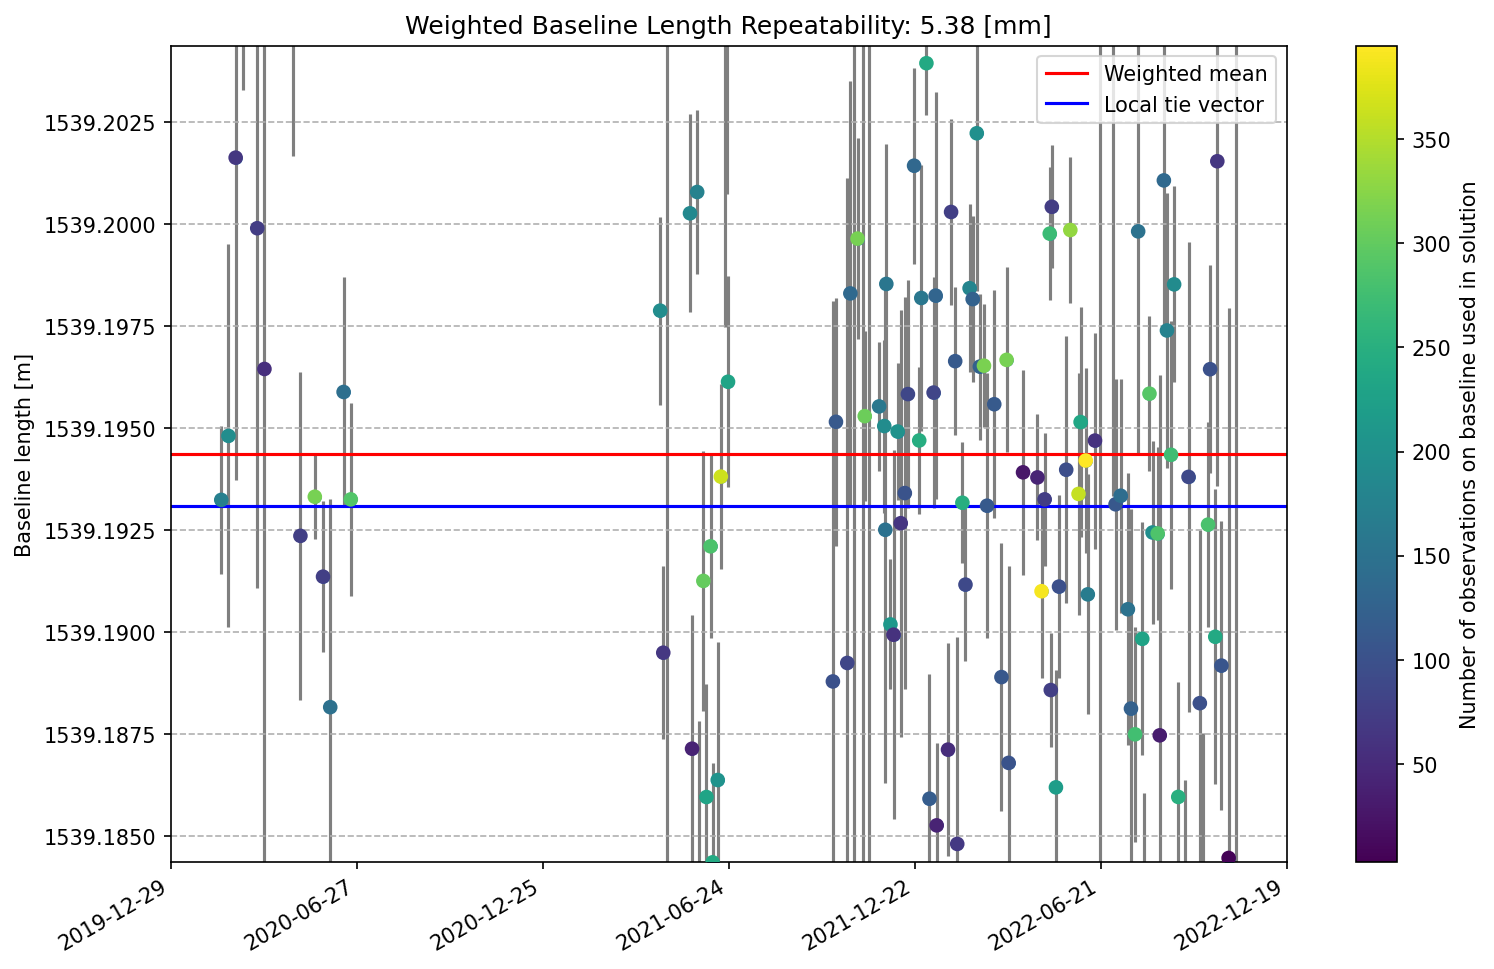
\includegraphics[width=16.0cm]{acnma01}
  \end{center}
  \caption{NYALES20-NYALE13S baseline lengths and weighted baseline length repeatability.The red line is the weighted mean of the
  individual solutions and the blue line is the local tie vector.}
  \label{fig:baseline}             
\end{figure*}   

\subsection{Working groups and projects}
The NMA analysis center has participated in several working groups and projects. 

\subsubsection{EU-VGOS}
The EU-VGOS project began in 2018 with the aim of using the VGOS infrastructure in Europe
to investigate methods for VGOS data processing. The project is now structured into Working Groups dealing
with operations (stations), e-transfer, correlation and post-processing, and analysis \cite{ivsgm2022-euvgos}.
NMA is participating in the analysis and operations working groups. One of the planned activities of the analysis working group
is to look closer at higher resolution troposphere estimates. Normal S/X sessions typically estimate the zenith
wet delay part of the troposphere every hour, but with the increased number of observations that VGOS is capable of
it should be possible to estimate troposphere parameters every 20 minutes. So far there is not too many sessions 
available in the EU-VGOS project. Other activities are also planned once different correlation methods are also tested.

\subsubsection{Six-hourly EOP Piecewise Linear
Offset Parameterization}
For a long time there has been a desire within the IVS to be able to estimate Earth Orientation Parameters
(EOP) at specific epochs to better align the results with EOP estimates from other space geodetic techniques.
In addition, it is interesting to investigate the feasibility of providing EOP estimates at a higher resolution
than 24 hours, which is common today. A project, lead by Axel Nothnagel, was established to look into this 
possibility. 

By modeling the EOP as continuous piecewise linear functions the project estimated the Earth Rotation Parameters
(ERP) polar motion and
UT1-UTC every six hours starting at midnight. The project used R1 sessions from 2020 and fixed the celestial pole
offset to an empirical model for 2020. The preliminary results showed that robust networks
with many observations per time interval are essential for this approach \cite{ivsgm2022-pwlo}.

\subsubsection{VLBI-scale}
When Zuheir Altamimi and his team created the ITRF2020 it became apparent that there is a drift in the 
VLBI scale after 2013.75 and the reasons for this drift are unknown. \cite{ivsgm2022-itrf2020}.
After the IVS GM 2022 the IVS directing board decided to create an ad hoc working group to investigate
this drift. The working group, by John 
Gipson, presented the preliminary results of this investigation at the Unified Analysis Workshop in 
Thessaloniki, Greece in October 2022 \cite{ivsnl-64}. The reasons for the drift in the VLBI scale is 
still not fully understood. Figure \ref{fig:scale} shows the scale drift computed with \textbf{Where}.

\begin{figure*}[htb!]         
  \begin{center}
  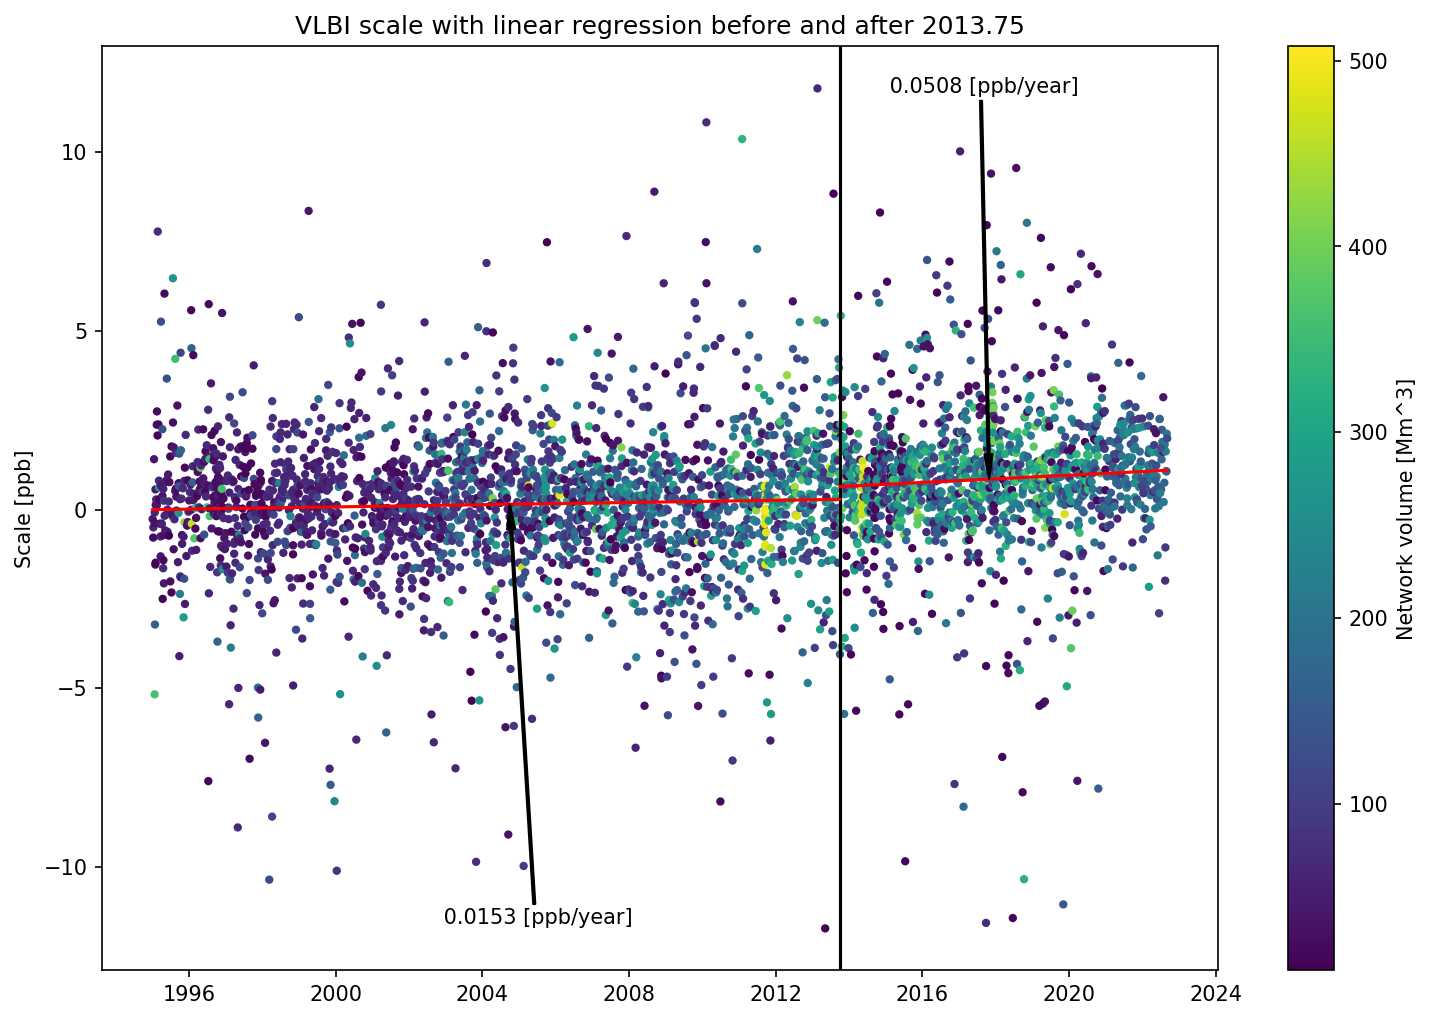
\includegraphics[width=16.0cm]{acnma02}
  \end{center}
  \caption{VLBI scale with regards to ITRF2020 computed with \textbf{Where}. The vertical black line is the epoch 2013.75 and
  the red lines are a linear regression of the sessions before and after 2013.75.}
  \label{fig:scale}             
\end{figure*}  

\subsection{Where}
At the beginning of 2023 a new naming convention for VLBI data files and a new format for the VLBI master file
will be implemented. This change required updates to \textbf{Where} and a new version have been made available 
to the community. 

To be able to participate in the working groups new features have been added to \textbf{Where}. Such as, the 
possibility to estimate parameters as continuous piecewise linear functions and computation of session-wise Helmert
parameters. 

In addition, several minor improvements and bugfixes have been implemented during 2021 and 2022.
%
\section{Current Status}
%
Currently, the NMA analysis center is working on the transition to the new naming convention. The transition seems
to be successful so far. 

A new operational solution, \texttt{2023a}, for the daily SINEX product is under way. This solution
will use ITRF2020 as a priori for station positions and velocities and include the new gravitational deformation models
that has been added since the prior solution.
%
\section{Future Plans}
%
NMA will continue with the operational analysis 24-hour sessions and contribute to the daily SINEX product. 
This also involves keeping \textbf{Where} up to date with current conventions. 

NMA also intends to continue participating in analysis working groups and projects when time allows and the scope of
 the work is within the capabilities of \textbf{Where} and the analysis center. 

As NYALE13N starts to observe more VGOS sessions these sessions are of special interest to the NMA analysis center
in the near future.
%
% Code to include a single column figure through \includegraphics.
% \begin{figure} and \end{figure} make this single column.
% If the figure is too wide, it will overwrite text in the other column.
% Figures should be centered through the latex \begin{center} and
% \end{center} commands.  
% Captions should be left-justified.  
% The class file will automatically perform the left-justification,
% if the caption is not included in the latex centering.
%
                  
%
% Code to use \includegraphics to include a figure that spans two columns. 
% \begin{figure*} and \end{figure*} will allow the figure to Span 
% two columns.  If the figure is too narrow, it will leave blank space 
% in the other column.
% Figures should be centered through the latex \begin{center} and
% \end{center} commands.  
% Captions should be left-justified.  
% The class file will automatically perform the left-justification,
% if the caption is not included in the latex centering.
%
%%\begin{figure*}[htb!]
% Please see the above figure example for naming conventions for the 
% figure file.
%%\begin{center}
%%\includegraphics[width=16.0cm]{ivs-br-template02.png}
%%\end{center}
% Please do not precede the caption by Figure 2.  
% Please just enter your desired text.
%%\caption{Example of figure from .png file.}
%%\label{second-unique-label}
%%\end{figure*}
%
% Code to include a single column table.
% Other table formats may be used also.  
% Tables should be centered through the latex \begin{center} and
% \end{center} commands.  
% Captions should be left-justified.  
% The class file will automatically perform the left-justification,
% if the caption is not included in the latex centering.
%
%%\begin{table}[htb!]
%%\caption{Caption for Table 1.}
%%\begin{center}
%%\begin{tabular}{|l|c|c|r|} \hline
%%Heading 1 & Heading 2 & Heading 3 & Heading 4\\
%%\hline
%%Value a1 & Value a2 & Value a3 &          \\
%%Value b1 &          & Value b3 & Value b4 \\
%%Value c1 & Value c2 & Value c3 &          \\
%%Value d1 & Value d2 & Value d3 & Value d4 \\
%%Value e1 & Value e2 & Value e3 & Value e4 \\
%%\hline
%%\end{tabular}
%%\end{center}
%%\label{third-unique-label}
%%\end{table}
%
% Code to include a two column table.
% Other table formats may be used also.  
% Tables should be centered through the latex \begin{center} and
% \end{center} commands.  
% Captions should be left-justified.  
% The class file will automatically perform the left-justification,
% if the caption is not included in the latex centering.
%
%%\begin{table*}[htb!]
%%\caption{Caption for Table 2.}
%%\begin{center}
%%\begin{tabular}{|l|c|c|r|l|c|c|r|} \hline
%%Heading 1 & Heading 2 & Heading 3 & Heading 4 & Heading 5 & Heading 6 & Heading 7 & Heading 8\\
%%\hline
%%Value a1 & Value a2 & Value a3 &          & Value a5 & Value a6 & Value a7 & Value a8 \\
%%Value b1 &          & Value b3 & Value b4 &          &          & Value b7 & Value b8 \\
%%Value c1 & Value c2 & Value c3 &          & Value c5 & Value c6 & Value c7 &          \\
%%Value d1 & Value d2 & Value d3 & Value d4 & Value d5 & Value d6 &          &          \\
%%Value e1 & Value e2 & Value e3 & Value e4 & Value e5 &          & Value e7 &          \\
%%Value f1 & Value f2 & Value f3 & Value f4 & Value f5 &          & Value f7 &          \\
%%Value g1 &          & Value g3 & Value g4 & Value g5 & Value g6 & Value g7 & Value g8 \\
%%\hline
%%Value h1 & Value h2 & Value h3 &          & Value h5 & Value h6 & Value h7 & Value h8 \\
%%Value i1 &          & Value i3 & Value i4 &          &          & Value i7 & Value i8 \\
%%Value j1 & Value j2 & Value j3 &          & Value j5 & Value j6 & Value j7 &          \\
%%Value k1 & Value k2 & Value k3 & Value k4 & Value k5 & Value k6 &          &          \\
%%Value l1 & Value l2 & Value l3 & Value l4 & Value l5 &          & Value l7 &          \\
%%Value m1 & Value m2 & Value m3 & Value m4 & Value m5 &          & Value m7 &          \\
%%Value n1 &          & Value n3 & Value n4 & Value n5 & Value n6 & Value n7 & Value n8 \\
%%\hline
%%Value o1 & Value o2 & Value o3 &          & Value o5 & Value o6 & Value o7 & Value o8 \\
%%Value p1 &          & Value p3 & Value p4 &          &          & Value p7 & Value p8 \\
%%Value q1 & Value q2 & Value q3 &          & Value q5 & Value q6 & Value q7 &          \\
%%Value r1 & Value r2 & Value r3 & Value r4 & Value r5 & Value r6 &          &          \\
%%Value s1 & Value s2 & Value s3 & Value s4 & Value s5 &          & Value s7 &          \\
%%Value t1 & Value t2 & Value t3 & Value t4 & Value t5 &          & Value t7 &          \\
%%Value u1 &          & Value u3 & Value u4 & Value u5 & Value u6 & Value u7 & Value u8 \\
%%\hline
%%Value v1 & Value v2 & Value v3 &          & Value v5 & Value v6 & Value v7 & Value v8 \\
%%Value w1 &          & Value w3 & Value w4 &          &          & Value w7 & Value w8 \\
%%Value x1 & Value x2 & Value x3 &          & Value x5 & Value x6 & Value x7 &          \\
%%Value y1 & Value y2 & Value y3 & Value y4 & Value y5 & Value y6 &          &          \\
%%Value z1 & Value z2 & Value z3 & Value z4 & Value z5 &          & Value z7 &          \\
%%\hline
%%\end{tabular}
%%\end{center}
%%\label{fourth-unique-label}
%%\end{table*}
%
% Please see the first two figures for detailed information
% about using figures.
%
%%\begin{figure*}[htb!]
%%\begin{center}
%%\includegraphics[width=16.0cm]{ivs-br-template03.pdf}
%%\end{center}
%%\caption{Example of figure from .pdf file.}
%%\label{fifth-unique-label}
%%\end{figure*}
%
% The acknowledgements section is optional.  If used, the section line should 
% be:
%      \section*{Acknowledgements}
%
%%\section*{Acknowledgements}

%%This section is optional.
%
% The bibliography section is optional.
%
% Here is a section with some examples.
% But the entries are free-format --- essentially,
%  \bibitem{unique-label}
%  text
%
%%%%%\begin{thebibliography}{99}
%%%%%\bibitem{Abbondanza2012}
%%%%%C.~Abbondanza and P.~Sarti.
%%%%%Impact of network geometry, observation schemes and telescope structure deformations on local ties:
%%%%%simulations applied to Sardinia Radio Telescope.
%%%%%\emph{Journal of Geodesy}, 86(3), doi:10.1007/s00190-011-0507-6, 181--192, 2012.
%%
%%%%%\bibitem{Artz}
%%%%%Thomas Artz, Judith Leek, Axel Nothnagel, and Maike Schumacher.
%%%%%VLBI Intensive Sessions Revisited.
%%%%%In D.~Behrend and K.~Baver, editors, \emph{International
%%%%%  VLBI Service for Geodesy and Astrometry 2012 General Meeting Proceedings},
%%%%%  NASA/CP-2012-217504, pages 276--280, 2012.
%%%%%%%
%%%%%\bibitem{VieVS}
%%%%%Matthias Madzak, Sigrid B\"ohm, Hana Kr\'asn\'a, and Lucia Plank.
%%%%%Vienna VLBI Software Version 2.1 User Manual
%%%%%Web document http://vievs.geo.tuwien.ac.at/fileadmin/editors/VieVS/documents/vievsDoc.pdf
%%%%%%
%%%%%\end{thebibliography} 
\begin{thebibliography}{99}

\bibitem{ivsgm2022-pwlo}
%A. Nothnagel1, S. B  ̈ohm1, R. Dach2, M. Glomsda3, H. Hellmers4, A.-S. Kirkvik5, T. Nilsson6, A. Girdiuk4, D. Thaller
A.\ Nothnagel et al, ``First Results of Project on Six-hourly EOP Piecewise Linear Offset Parameterization'',
In IVS 2022 General Meeting Proceedings, edited by K.\ Armstrong, D.\ Behrend, and K.\ Baver,
NASA/CP-20220018789, 2023
\bibitem{ivsgm2022-euvgos}
E.\ Albentosa et al. ``Current Status of the EU-VGOS Project'',
In IVS 2022 General Meeting Proceedings, edited by K.\ Armstrong, D.\ Behrend, and K.\ Baver,
NASA/CP-20220018789, 2023
\bibitem{ivsgm2022-nyal}
Susana Garcia-Espada et al. ``Status at Ny-Ålesund Geodetic Earth Observatory'',
In IVS 2022 General Meeting Proceedings, edited by K.\ Armstrong, D.\ Behrend, and K.\ Baver,
NASA/CP-20220018789, 2023
\bibitem{evga-baseline}
A.-S. Kirkvik et al, ``First results from the new station NYALE13S'', In Proceedings of the 24th 
European VLBI Group for Geodesy and Astrometry Working Meeting. Edited by Rudiger Haas, 2019.
ISBN: 978-91-88041-41-8.
\bibitem{evga-itrf2020}
%Hendrik Hellmers, Sadegh Modiri, Sabine Bachmann, Daniela Thaller, Mathis Bloßfeld, Manuela Seitz, John Gipson
H. Hellmers et al, ``Combined IVS contribution to the ITRF2020'', In Proceedings of the 24th 
European VLBI Group for Geodesy and Astrometry Working Meeting. Edited by Rudiger Haas, 2019.
ISBN: 978-91-88041-41-8.
\bibitem{ivsgm2022-itrf2020}
%Zuheir Altamimi1, Paul Rebischung1, Xavier Collilieux1,2, Laurent M  ́etivier1, Kristel Chanard1
Z. Altamimi et al, ``ITRF2020 and the IVS Contribution'', 
In IVS 2022 General Meeting Proceedings, edited by K.\ Armstrong, D.\ Behrend, and K.\ Baver,
NASA/CP-20220018789, 2023
\bibitem{ivsnl-64}
https://ivscc.gsfc.nasa.gov/publications/newsletter/issue64.pdf
\bibitem{biennial-acnma2019}
A.-S. Kirkvik, ``Norwegian Mapping Authority Analysis Center Biennial Report 2019--2020'', 
In International VLBI Service for Geodesy and Astrometry 2019+2020 Biennial Report, edited by 
D.\ Behrend, K.\ L.\ Armstrong, and K.\ D.\ Baver,
 NASA/TP-20210021389, 2021. 
%D.~Behrend, ``Coordinating Center Report'',
%In K.\ D.\ Baver, D.\ Behrend, and K.\ Armstrong, editors, International
%VLBI Service for Geodesy and Astrometry 2012 Annual Report,
%NASA/TP-2013-217511, pages 55--57, 2013.

\end{thebibliography}
%
\end{document}
